%% GENERATED by tools/from_docs.py from stepss-docs. Do not edit by hand:
%% edit the page named below in stepss-docs and regenerate.
%% source: stepss-docs/src/content/docs/gui/running.mdx

\chapter{Running a simulation in STEPSS GUI}\label{doc:gui-running}

This walks one case end to end: the Kundur two-area system, a load step, and the
inter-area oscillation that follows. It needs no data of your own, because the case
ships with the application.

If you have not opened it yet, \hyperref[doc:gui-first-run]{First Run} covers \textbf{File, Open
Examples}. Pick \textbf{Kundur two-area} and come back.

\section{1. Check what was loaded}\label{gui-running:check-what-was-loaded}

Opening the example fills the case in, so there is nothing to do here but look.
\textbf{System Data} should hold three system data files and one disturbance file:

{\def\LTcaptype{none} % do not increment counter
\begin{small}\begin{longtable}[]{@{}
  >{\raggedright\arraybackslash}p{(\linewidth - 6\tabcolsep) * \real{0.2834}}
  >{\raggedright\arraybackslash}p{(\linewidth - 6\tabcolsep) * \real{0.2587}}
  >{\raggedright\arraybackslash}p{(\linewidth - 6\tabcolsep) * \real{0.4579}}
@{}}
\toprule\noalign{}
\begin{minipage}[b]{\linewidth}\raggedright
Slot
\end{minipage} & \begin{minipage}[b]{\linewidth}\raggedright
File
\end{minipage} & \begin{minipage}[b]{\linewidth}\raggedright
What it holds
\end{minipage} \\
\midrule\noalign{}
\endhead
\bottomrule\noalign{}
\endlastfoot
System data 1 & \texttt{lf.dat} & The network and the power-flow data \\
System data 2 & \texttt{dyn.dat} & The dynamic models: machines, exciters, governors, loads \\
System data 3 & \texttt{solveroptions.dat} & \hyperref[ch-settings]{Solver settings} \\
Disturbance & \texttt{disturb.dst} & What happens, and when \\
\end{longtable}\end{small}
}

The disturbance is three lines, and worth reading before running anything:

\begin{Verbatim}
  0.000 CONTINUE SOLVER BD 0.01 0.0001 0. ALL
  1.000 CHGPRM INJ L9 Po +0.5 0
 60.000 STOP
\end{Verbatim}

At \texttt{t\ =\ 1\ s} the active power set point of load \texttt{L9} is stepped by \texttt{+0.5} pu, and
the run ends at 60 s. \hyperref[ch-disturb]{Disturbances} is the reference
for these records.

\section{2. Choose what to record}\label{gui-running:choose-what-to-record}

On \textbf{Observables}, \texttt{obs.dat} is already loaded and \textbf{Save output trajectory} is
already checked, which is the pair you need: the trajectory is the file the curves
come from, and the observables file says what goes into it.

If you want to watch the run as it happens, set a \textbf{runtime observable}. Machine
speed of \texttt{G1} and the voltage of bus \texttt{9} are good choices for this case. A refresh
interval of 1 second is plenty.

\begin{docsnote}{Note}

This case sets \texttt{\$GP\_REFRESH\_RATE\ 1.0} in \texttt{solveroptions.dat} already. The field on
the tab is the same setting, and either place works.

\end{docsnote}

\section{3. Solve the power flow}\label{gui-running:solve-the-power-flow}

On \textbf{Power Flow Simulation}, click \textbf{Run power flow}.

\begin{figure}[htbp]
\centering
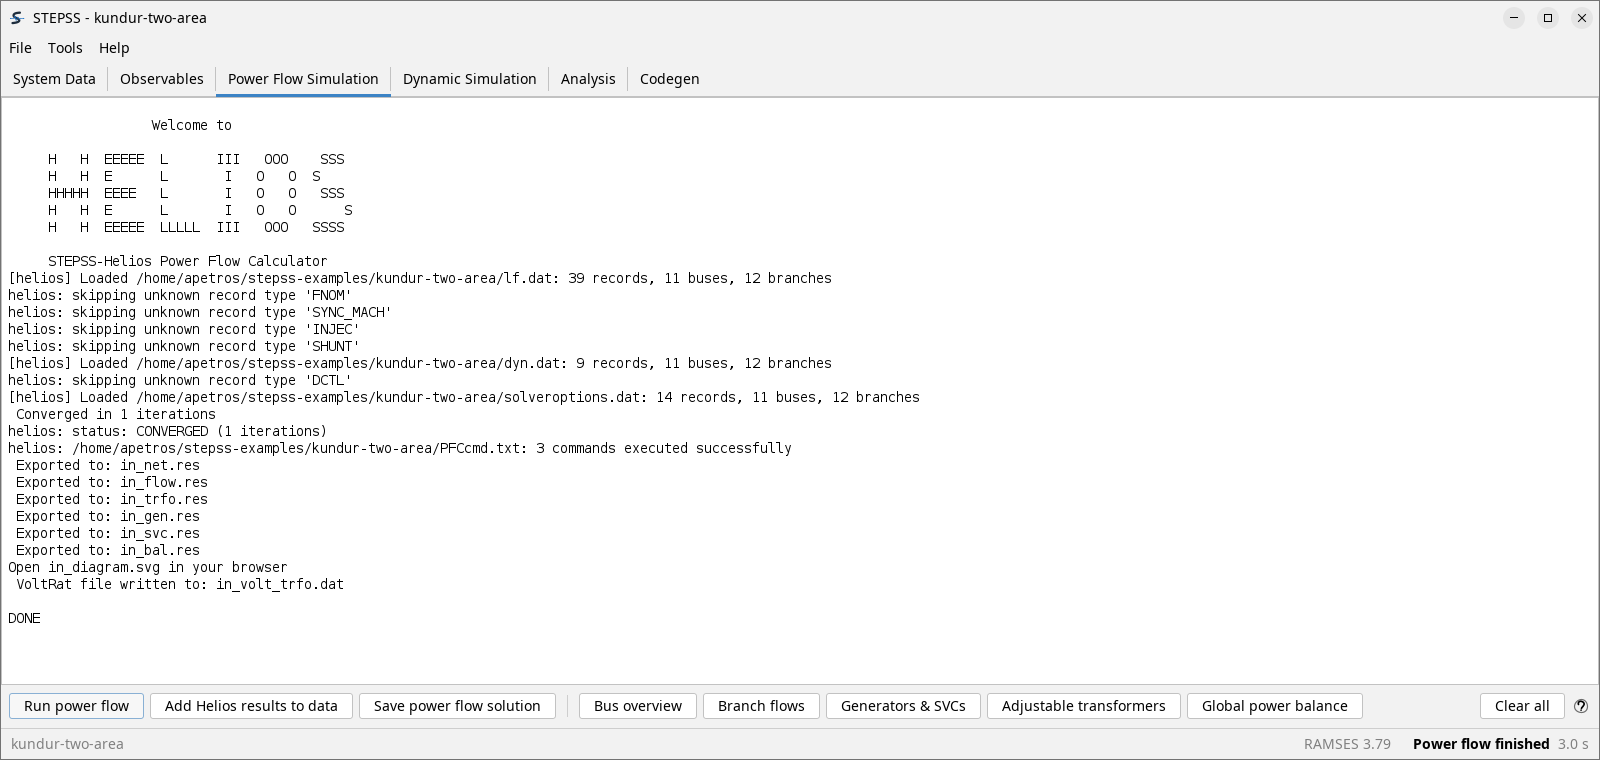
\includegraphics[width=0.98\linewidth]{figures/gui-power-flow-light}
\caption{The Power Flow Simulation tab after a successful run on the Kundur case.}
\end{figure}

Read the balance at the bottom before going on. For this case the load totals
2734 MW against 2819 MW of generation, the difference being the 85.1 MW of network
losses. A balance that does not add up, or a generator sitting on a reactive limit,
is a problem to fix here rather than to discover halfway through a dynamic run.

The five inspection buttons beside \textbf{Run power flow} become available now:
\textbf{Bus overview}, \textbf{Branch flows}, \textbf{Generators \& SVCs}, \textbf{Adjustable
transformers} and \textbf{Global power balance}, each of which writes its table
into the same pane. \hyperref[doc:gui-interface]{The Interface}
shows what each one produces.

\section{4. Run the simulation}\label{gui-running:run-the-simulation}

On \textbf{Dynamic Simulation}, click \textbf{Run dynamic simulation}.

\begin{figure}[htbp]
\centering
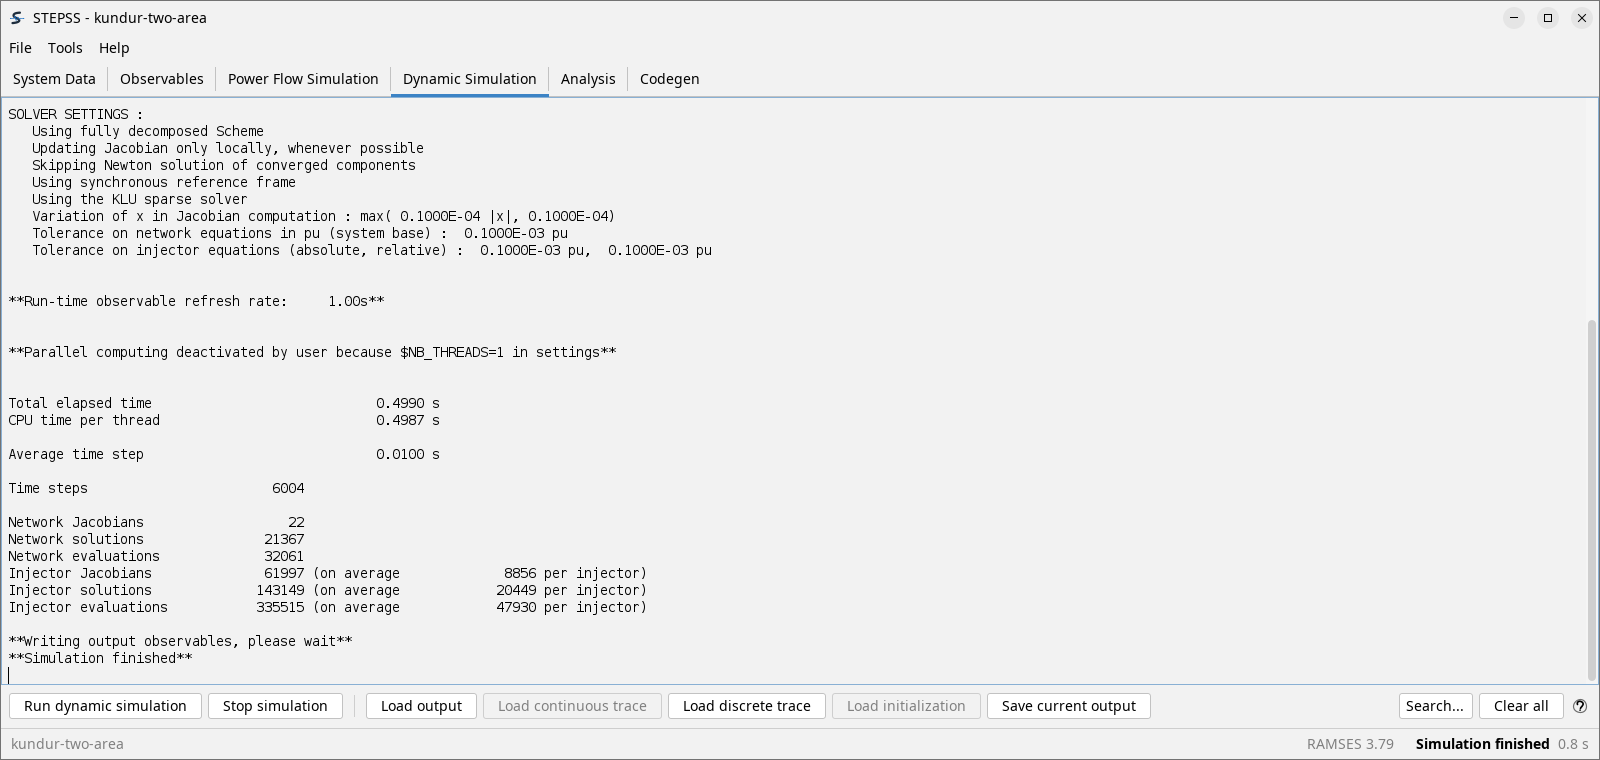
\includegraphics[width=0.98\linewidth]{figures/gui-dynamic-simulation-light}
\caption{The Dynamic Simulation tab after a completed run.}
\end{figure}

The pane opens with the settings actually in force, which is the place to confirm
that the case is doing what you meant. This one reports the synchronous reference
frame, the KLU sparse solver, local Jacobian updates, and that converged components
are skipped.

It also says \textbf{parallel computing deactivated by user}, because the case sets
\texttt{\$NB\_THREADS\ 1}. That is a property of this example, not a limit of the engine.

60 seconds of system time takes well under a second of wall time here, in 6004
steps. The counts below are the cost of the run: how often the network and the
injector Jacobians were rebuilt and solved. They are what to watch when a bigger
case gets slow.

If you set the runtime observables in step 2, a \textbf{Run-time curves} window drew
them as the run advanced and is still up when it finishes; see
\hyperref[doc:gui-first-run]{Real-time plotting}.

\section{5. Extract the curves}\label{gui-running:extract-the-curves}

On \textbf{Analysis}, click \textbf{Extract curves}. The picker reads the trajectory and
offers whatever the observables file recorded.

\begin{enumerate}
\def\labelenumi{\arabic{enumi}.}
\item
  Set \textbf{Category} to \texttt{SYNC}, which lists the four synchronous machines.
\item
  Select \texttt{G1} and set \textbf{Observable} to \texttt{active\ power\ produced\ (MW)}, then click
  \textbf{Add}.
\item
  Select \texttt{G3}, leave the observable as it is, and \textbf{Add} again.
\item
  Click \textbf{Plot}.
\end{enumerate}

\begin{figure}[htbp]
\centering
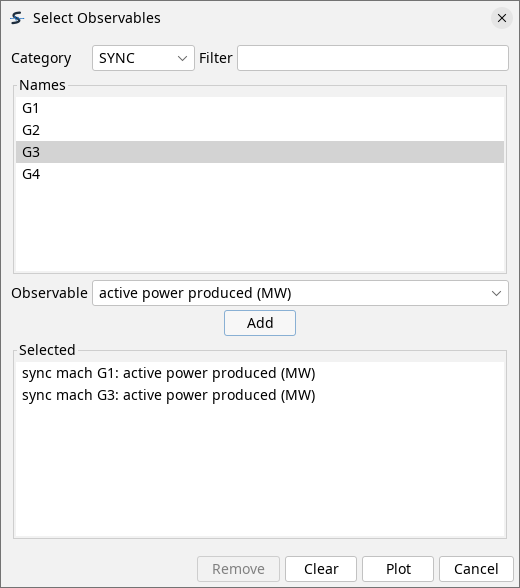
\includegraphics[width=0.98\linewidth]{figures/gui-select-observables-light}
\caption{The Select Observables dialog with category SYNC chosen, machines G1 to G4 listed, and two entries queued in the Selected list: active power produced in MW for sync mach G1 and for sync mach G3.}
\end{figure}

\texttt{G1} and \texttt{G3} are the point of the exercise: one sits in each area, so putting them
on the same axes shows the oscillation \emph{between} the areas rather than within one.

\section{6. Read the result}\label{gui-running:read-the-result}

\begin{figure}[htbp]
\centering
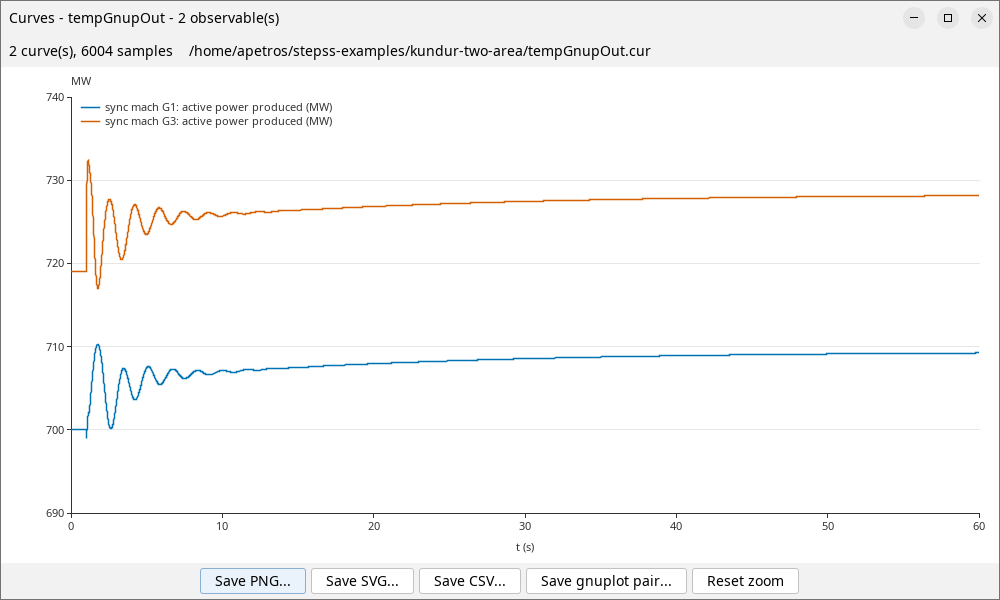
\includegraphics[width=0.98\linewidth]{figures/gui-plot-light}
\caption{Active power produced by generators G1 and G3 against time, drawn as two curves on one set of axes with a legend naming each.}
\end{figure}

Three things to see in it.

The two machines swing \textbf{in opposition}. When \texttt{G3} is at a peak, \texttt{G1} is near a
trough. That anti-phase pattern is what makes this an inter-area mode rather than a
local one: the two areas are oscillating against each other across the weak tie.

The period is about 1.4 seconds, so roughly 0.7 Hz, which is the range inter-area
modes normally sit in.

The oscillation \textbf{decays}, and after about ten seconds both machines settle a few
megawatts above where they began, sharing the extra load. That decay is the damping,
and it is the quantity the next section changes.

\section{Try it with the stabiliser out}\label{gui-running:try-it-with-the-stabiliser-out}

The example ships a second dynamic file, \texttt{dyn\_noPSS.dat}, identical to \texttt{dyn.dat}
except that the power system stabiliser gain is set to zero.

On \textbf{System Data}, load \texttt{dyn\_noPSS.dat} into slot 2 in place of \texttt{dyn.dat}, then
repeat steps 3 to 6. Everything else stays as it is.

The mode is the same and its frequency barely moves, but it is far less damped.
Comparing the two runs is the standard demonstration of what a PSS is for, and it
is why the case ships both files.

\section{Where to go next}\label{gui-running:where-to-go-next}

\begin{itemize}
\tightlist
\item
  \hyperref[ch-disturb]{Disturbances}, to change what happens and when
\item
  \hyperref[ch-settings]{Solver Settings}, to change how it is solved
\item
  \hyperref[doc:eigenanalysis]{Eigenanalysis}, to get this mode's frequency and
  damping as numbers instead of reading them off a curve
\item
  \hyperref[doc:ts-kundur]{Kundur Two-Area System}, the system itself in detail
\item
  \hyperref[doc:py-examples]{STEPSS in Python}, the same run as a script
\end{itemize}
